%File: formatting-instruction.tex
\documentclass[letterpaper]{article}
\usepackage{aaai}
\usepackage{times}
\usepackage{helvet}
\usepackage{courier}
\usepackage{url}
\usepackage{graphicx}
\usepackage{amsmath}
\usepackage{latexsym}
\usepackage{amssymb}
\usepackage{multirow}
\newtheorem{definition}{Definition}
\frenchspacing
\setlength{\pdfpagewidth}{8.5in}
\setlength{\pdfpageheight}{11in}
\pdfinfo{
/Title (Insert Your Title Here)
/Author (Put All Your Authors Here, Separated by Commas)}
\setcounter{secnumdepth}{0}  
 \begin{document}
% The file aaai.sty is the style file for AAAI Press 
% proceedings, working notes, and technical reports.
%
\title{From Interests to Opinions: \\Modelling Subjectivity for Retweeting Analysis}
\author{Songxian Xie, Jintao Tang \and Ting Wang\\
School of Computer, National University of Defense Technology, Changsha, P.R. China\\
\AND Ruili Wang\\
School of Engineering and Advanced Technology, Massey University, Auckland, New Zealand\\
\AND Kewen Wang\\
School of Information and Communication Technology, Griffith University, Brisbane, QLD 4111 Australia\\
}
\maketitle
\begin{abstract}
\begin{quote}
Social media such as Twitter provides researchers with abundant User-Generated Content (UGC) for analyzing users' online behaviors.  In this paper, we focus on retweeting behavior, which is one of the key mechanisms of information dissemination on Twitter. 
User modelling has been proved to be effective in previous researches. However few studies have investigated the subjectivity of users. 
Motivated by psychological researches, we propose a novel subjectivity model by combining both topic-of-interests and opinions articulated in UGC. 
We also define a novel weighting function to measure the subjectivity similarity, and demonstrate that a user is more likely to retweet a message because of approximate subjectivity similarity.  
In the experiments, the subjectivity similarity is verified to be correlated with retweeting behavior by means of ANOVA test. 
When comparing with other topic-based models in retweeting prediction, our model outperforms other models with best accuracy. Our model gives significant accuracy improvement over an off-the-shelf predicting model considering other factors.
\end{quote}
\end{abstract}

\section{Introduction}
\label{introduction}
\noindent Microblogging has become a center of attention in the area of social networking due to the amount of users it has attracted and the volume of messages it produces daily. 
Microblogging services such as Twitter appear to play an important role in the process of information dissemination on the Internet, making it possible for messages to spread virally in a matter of minutes. 
The retweeting convention and complex network of Twitter provide an unprecedented mechanism for the spread of information despite the restricted length of a single message (i.e. tweet). 
Actually almost a quarter of the tweets are retweeted from other users \cite{yang2010understanding}. 
Understanding how retweeting behavior works can help explaining information dissemination on Twitter. 

There have been many studies trying to identify factors that influence whether a tweet will be retweeted \cite{boyd2010tweet,kwak2010twitter}. However few studies have investigated the subjective motivation of a user to retweet a message. 
The subjective initiative nature of human determines that his behavior pattern is subjectivity driven. Psychological researchers have identified subjectivity as the underlying factor that influences human's behaviors \cite{moore2008awareness}. 
Also according to theory of \textbf{Biased Assimilation}, people tend to choose and disseminate information according to their own biased subjectivity \cite{Hyman2000}. 
Users receive thousands of tweets on different topics every day, whether a tweet will be retweeted will depend on the subjective choice of users. 
From the point of a user, retweeting is a process that includes reading the tweet, evaluating the content and deciding whether to share. The crucial part is to evaluate whether a tweet contains information interesting to the user who might find that it is worthy to be shared.  
Therefore modelling the subjective motivation of users will provide an important perspective for retweeting behavior analysis. 
This research is motivated by a desire to find what drives the subjective users of social networks to disseminate information they come across. 

Previous studies on retweeting analysis have shown that an enriched user model gives coherent and consistent explanation for retweeting motivation \cite{macskassy2011people,feng2013retweet}. 
Specifically, researchers have tried to model users from four types of information:
profile features (``\textbf{Who you are}"), tweeting behavior (``\textbf{How you tweet}"), linguistic content (``\textbf{What you tweet}") and social network (``\textbf{Whom you connect}") \cite{pennacchiotti2011machine}. 
Especially topics encapsulated in rich linguistic content of a user have been proved consistently dependable for behavior analysis \cite{petrovic2011rt}. However no studies have considered how to model the subjective aspect (``\textbf{what's your opinions}") when modelling a user.  In this paper, we propose a novel method to model sujectivity of a user(we name it subjectivity model) by combining both the topics and opinions.

Social media is a platform where different opinions are presented by allowing users gennerate contents on topics they are interested in. 
The subjectivity of a user is encoded in the User-Generated Content (UGC) on Twitter. 
Therefore, we explore the tweets a user has published to establish the subjectivity model. 
For the retweeting analysis problem, we assume the probability a user retweets a message could be evaluated with subjectivity similarity measurement. 
We design a novel weighting function to measure the subjectivity similarity, and propose three subjectivity similarities among a tweet, its author and followers to analyze the motivation of retweeting behaviors. 
Expertiments on Twitter dataset show that retweeting behaviors are correlated with all three subjectivity similarities, our subjectivity model outperforms topic-based user model for retweeting prediction, and the subjectivity similarities significantly improve the performance of an off-the-shelf predicting model considering other factors. 

The rest of the paper is organized as follows: we give the definition and establishment details of the proposed subjectivity model in the next section, and in section 3 the subjectivity similarity is defined and specified for the retweeting analysis problem, experiments of quantitative evaluation is carried out in section 4, the related works are described in section 5 and Section 6 summarizes the paper and points out future work.

\section{Subjectivity Model}
\label{subjectivemodel}

Subjectivity has been extensively studied by psychologists to characterize the personality of a person based on his historic behaviors and remarks \cite{engbert2007agency}. 
Linguists define the subjectivity of language as speakers always show their perspectives, attitudes and sentiments to events, people, topics, and entities in their linguistic contents \cite{stein2005subjectivity}. 
How to computationally model the subjectivity of a user is still a challenging problem. 
The advent of online social media such as Twitter has given a new layout to the challenge.  
Twitter allows users to show their personal subjectivity by publishing short messages, which provides researchers with data resources to model the subjectivity of users.
First of all, we give a formal definition of the subjectivity model under the context of Twitter.

\subsection{Definition}
\label{definition}

Let $G=\left( V,E \right) $ denotes a social network, where $ V $ is a set of users on Twitter, and $ E\subset V\times V $ is a set of following relationships between users. For each user $ u \in V $, there is a tweets collection $ M_{u} $ denotes his message history. We assume there is a topic space $ T $ containing all topics they talk about, and a sentiment valence space $ O $ to evaluate their opinions towards these topics. 
For the ``subjectivity'' of a user $ u  \in V $, we refer to both topics of interest and opinions articulated in his tweets collection $ M_{u} $.  
\begin{definition}[Subjectivity Model]
The subjectivity model $ P \left( u \right) $ of user $ u $, is the combination of topics $\left\lbrace  t_{i} \right\rbrace $ the user talks about in topic space $T$ and the user's opinions ${o_{i}}$ towards each topic evaluated in sentiment valence space $ O $. 
\begin{equation}
\label{usermodel}
P \left( u \right) = \lbrace \left( t_{i}, w_{u} \left( t_{i} \right), d_{u,t_{i}} \left( o_{i} \right) \right) \,\vert  t_{i} \in T, \, o_{i} \in O \rbrace
\end{equation}
where:
\begin{itemize}
\item with respect to user $ u $, for each topic $t_{i} \in T$, its weight $ w_{u} \left( t_{i} \right)$ represents the distribution of the user's interests on it, subject to $ \sum_{i=1}^{|T|}w_{u} \left( t_{i} \right)=1 $.
\item opinion of the user towards topic $t_{i}$ is modelled as a topic-dependent sentiment distribution  $d_{u,t_{i}} \left( o_{i} \right)$ over sentiment valence space $ O $.
\end{itemize}
\end{definition}
Figure~\ref{fig0} is a visualized subjectivity model of a user in a $ [0,100] $ topics space and a $ [0,8] $ sentiment valence space. 
\begin{figure}[htb]
%\centering
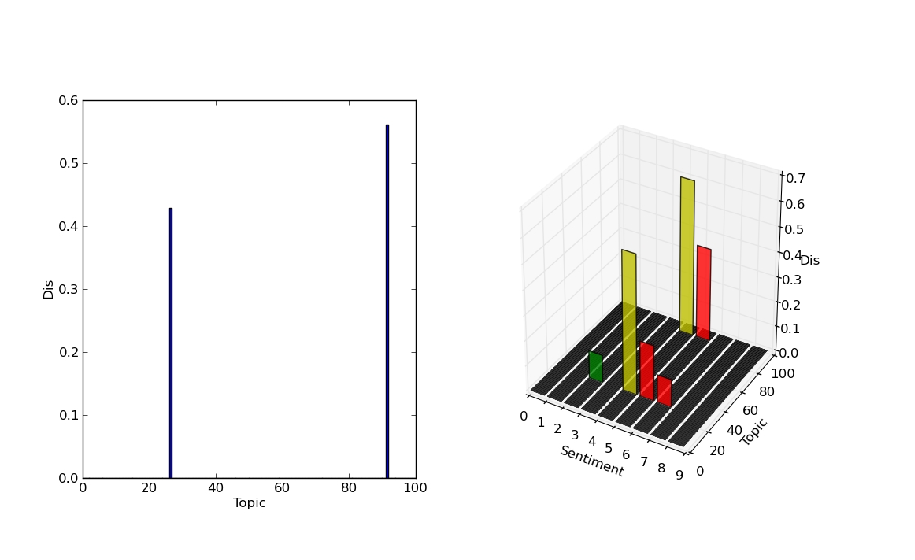
\includegraphics[width=3.8in,height=2.0in]{fig1.pdf}
\caption{The left subgraph denotes two topics a user tweets about with weights $ \left( w_{u}\left( t_{23} \right)=0.43, w_{u}\left( t_{86} \right)=0.57\right)  $. the right subgraph denotes opinions towards two topics: for topic 23, $ ( d_{u,t_{23}} \left( o_{2} \right)=0.1, d_{u,t_{23}} \left( o_{4} \right)=0.5,d_{u,t_{23}} \left( o_{5} \right)=0.3,d_{u,t_{23}} \left( o_{6} \right)=0.1) $; for topic 86, $ \left( d_{u,t_{86}} \left( o_{4} \right)=0.66, d_{u,t_{86}} \left( o_{5} \right)=0.34 \right) $.}
\label{fig0}
\end{figure}

\subsection{Establishment of Subjectivity Model}
\label{establishment}

The definition of a subjectivity model is in an abstract form by using latent concepts of topics and opinions,  which need to be derived from the message histories of all users $ M=\lbrace M_{u}\vert u \in V\rbrace$  

\subsubsection{Topic Analysis}
\label{topic}

Topic analysis for all users in a global network on Twitter is a nontrivial task. 
There are millions of users and billions of tweets associated with these users. The effectiveness and efficiency of the topic analysis algorithm is a big problem.
However, the ``follow'' relationship on Twitter is a strong indicator of a phenomenon called ``homophily'', which has been observed in many social networks \cite{mcpherson2001birds}.
Homophily implies that a user follows another user because of sharing common interests. 
According to the principle of homophily, we put forwards the concept of \textbf{Local Topic Space} by combining topic analysis and network topology on Twitter: 
\begin{definition}[Local Topic Space]
\label{local}
Let $G=\left( V,E \right) $ denotes global social network, for a user $ u \in V $, we use $ G_{u}^{\tau} \subseteq G$ 
to denote $ u $'s $ \tau $-ego network, where $ \tau $-ego network means subnetwork formed by $ u $'s $ \tau $-hop 
friends in the network $ G $, and $ \tau \geqslant 1 $ is a tunable integer parameter to control the scale of the ego network. 
In the $ \tau $-ego network of $ u $, all users concentrate on limited topics derived from the content generated by them, and these topics form a local topic space $ T_{u} $.
\end{definition}

Previous studies have tried to identify topics from tweets by finding key words \cite{chen2010short}, extracting  entities \cite{abel2011analyzing} or linking tweets to external knowledge categories \cite{macskassy2011people}. Works also show that topic models such as \textbf{Latent Dirichlet Allocation (LDA)} model \cite{blei2003latent} are more effective in identifying topics from short and informal social media language \cite{hong2010empirical}, so we adopt the user-level LDA model for topic analysis. 
However, the LDA model is adapted to our local topic space assumption, and the relatively tiny size and topic homophily of an ego network lower the impact of data sparsity and degrade the calculation complexity of LDA.
 
\subsubsection{Opinion Mining}
\label{opinion}

In the Natural Language Processing area, opinion mining or sentiment analysis is formally defined as the computational study of sentiments and opinions about topics expressed in a text \cite{liu2012sentiment}. Opinions are often regulated as sequential discrete values to represent sentiment strength (for example: 0 stands for negative and 1 for positive). Sentiment analysis researches have dived into the social media language and provided effective sentiment analysis tools \cite{thelwall2010sentiment,hu2013unsupervised}. In this work,we just make use of the off-the-shelf work of sentiment analysis.
The SentiStrength package has been built to cope with sentiment analysis in short informal text of social media \cite{thelwall2010sentiment}. 
It assigns two values to each tweet standing for sentiment strengths: a positive and a negative sentiment measurement, with $ \left[ -5,-1 \right]  $ denoting negative and $ \left[ 1,5 \right]  $ denoting positive sentiment strength, which can be used to catch fine opinion distributions in a user's subjectivity model.  
For the convenience of distribution calculation, we map the output of SentiStrength to a single value in sentiment valence space $ \left[ 0, 8 \right] $ as follows:
\begin{equation}
\label{opinionmap}
o= \left\{ 
\begin{array}{lll}
{p+3} & if \vert p \vert > \vert n \vert \\
{n+5} & \text{if } \vert n \vert > \vert p \vert \\
{4}  & \text{if } \vert p \vert = \vert n \vert
\end{array}
\right.
\end{equation}
where $ p $ denotes the positive sentiment strength and $ n $ denotes negative sentiment strength. 

\subsubsection{Concreting Subjectivity Model}
\label{concrete}
 
As Definition~\ref{local} describes, a $ \tau $-ego network $ G_{u}=\left( U,E_{u} \right)  $ for a user $ u $ can be extracted from global network. 
Then the subjectivity model of each user $ u \in G_{u} $ can be concreted within the ego network. 
$ M_{u}=\left\lbrace m_{i} \vert i \in \left[ 1, \cdots, N \right]  \right\rbrace$ denotes tweets set published by user $ u $. A Local Topic Space $ T_{u}=\left\lbrace t_{i} \vert i=1, \cdots, K \right\rbrace $ can be constructed using LDA topic model with a single document representing all concatenated tweets in $ M_{u} $.
The topic model is built with the parameter $ \theta_{u} $\ representing the distribution of user $ u $ over topics he talks about. Simultaneously SentiStrength is applied to each tweet $ m \in M_{u} $ and outputs sentiment strength $ s_{m} $. 
subjectivity model of user $ u $ is built as follows:
\begin{itemize}
\item Firstly, the corresponding parameter $ \theta_{u} $ of topic model for user $ u $ can be regarded as his topic distribution in the Local Topic Space $ T_{u} $, and the topics he talks about are $ Z_{u}= \left\lbrace z \vert p\left( z \vert \theta_{u}\left( z \right)  \right)>0 \right\rbrace $.
\item Secondly, the topic model is applied to each tweet $ m $ to identify topics it talks about, denoted as $ Z_{m} =\left\lbrace z_{m} \vert p\left( z_{m} \vert \theta, \beta, Z_{u} \right)>0 \right\rbrace $.
\item Thirdly, the opinion distribution of user $ u $ towards topic $ t \in Z_{u} $ could be calculated as: 
\begin{equation}
\label{opinionall}
d_{u,t}\left( o \right) = \left\lbrace \dfrac{N_{o}}{\sum_{o \in O} N_{o}} \vert O=\left[ 0,8 \right] \right\rbrace 
\end{equation}
where $ N_{o} $ is the number of times user $ u $ expresses an opinion towards topic $ t $ with sentiment strength $ o $, which could be calculated as:
\begin{equation}
\label{opinion1}
N_{o}=\sum_{m \in Mu} I\left( s_{m} \right) , \text{ if } s_{m}=o \& t \in Z_{m}
\end{equation}
\begin{equation}
\label{opinion2}
I\left( s_{m} \right)=\left\{
\begin{array}{ll}
{1} & \text{if } s_{m}=o \& t \in Z_{m}\\
{0} & \text{else}
\end{array}
\right.
\end{equation}
For simplicity, it is postulated that the sentiment of each tweet $ s_{m} $ is related to all topics it talks about in $ Z_{m} $. As a future work, we will adopt more sophisticated method to identify opinion towards each topic in a tweet.
\end{itemize}

\section{Retweeting Analysis With Subjectivity Model}

Many factors have been proved to affect retweeting behavior \cite{suh2010want,macskassy2011people,comarela2012understanding}, however few researches have investigated the subjective motivation of a user to retweet a message. 
Apart from the context constraints, a tweet is more likely to be retweeted by a user who find its content worth to. 
Therefore, we are not interested in modelling the tweet by itself as other researches \cite{naveed2011searching,pfitzner2012emotional}, but the underlying reasons why a user want to disseminate it based on his subjective initiative. 
We assume that if a tweet is published, all followers of its author will receive it in time, and followers are likely to retweet it if they find it worthwhile. 
Under such assumption, we investigate the retweeting problem within a 1-ego network for the author of target tweets. 
In the ego network, the relation among the tweet, its author and followers can be illustrated as Figure~\ref{fig1}.
\begin{figure}[htb]
%\setlength{\belowcaptionskip}{-0.2cm} 
\centering
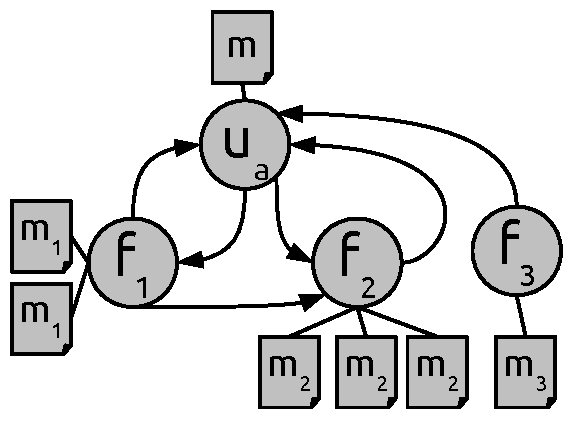
\includegraphics[width=1.8in,height=1.6in]{ego.pdf}
%\vspace{-4em}
\caption{Illustration of relations among tweet, author and followers. Author is denoted as $ u_{a} $, tweet as $ m $, followers as $ f_{i} $ and tweets of follower $ f_{i} $ as $ m_{i} $. An directed edge $ \left( f_{i},u_{a} \right)  $ means that $ f_{i} $ is exposed to the messages published by $ u_{a} $.}
\label{fig1}
\end{figure}

\subsection{Problem Formulation}
\label{formulation}

The retweeting analysis problem can be formulated as follows:
For each target tweet $ m $, let $ F $ denotes the followers who receive $ m $ by following its author $ u_{a} $, and for each user $ u \in F \cup \left\lbrace u_{a} \right\rbrace  $, let $ M_{u} $ denotes a tweet collection $ u $ has published. 
For each follower $ u_{f} \in F $, we can define a quadruple $ <u_{f}, u_{a}, m, r_{f}>  $: 
\begin{itemize}
\item $ r_{f} $ is a binary label indicating whether $ m $ is retweeted by $ u_{f} $.
\item Firstly our work focuses on building subjectivity model $ P\left( u \right)  $ for each user $ u \in F \cup \left\lbrace u_{a} \right\rbrace $ in the ego network with all tweets collections $ M=\left\lbrace M_{u} | u \in F \cup \left\lbrace u_{a} \right\rbrace  \right\rbrace  $.
\item Then we investigate the relation between the subjectivity of a user and his retweeting behavior to predict $ r_{f} $ by calculating subjectivity similarities between tweet $ m $, its author $ u_{a} $ and follower $ u_{f} $. 
\end{itemize}

\subsection{Subjectivity Similarity}
\label{similarity}

We assume that if the tweet content and the subjectivity of a user are similar enough in terms of topics and opinions, the user will have a very high probability to adopt retweeting behavior. 
With the subjectivity models estabilshed for the author and followers, the subjective decision-making procedure can be simulated by calculating the subjectivity similarity between the tweet and users. 
In this section, we define a novel similarity measurement to quantify the subjectivity similarity, which can be divided into topic similarity and opinion similarity. 
For the calculating convenience, the tweet $ m $ is analyzed and a ``subjectivity model'' is established for  $ m $ according to the procedure for users. 
Thus the subjectivity similarity calculation for tweet and user is identical with subjectivity similarity calculation between users.
 
\subsubsection{Topic Similarity}
\label{topsim}

The similarity between two topic distributions can be calculated with methods such as the cosine distance \cite{cha2007comprehensive} or the Jensen-Shannon Divergence \cite{weng2010twitterrank} with satisfactory results.
We adopt a cosine distance to measure the topic similarity because it performs better than other measurements in our research settings. It is defined as:
\begin{equation}
sim_{topic}=\dfrac{\theta_{m} \cdot \theta_{u}}{\parallel \theta_{m} \parallel \parallel \theta_{u} \parallel}
\end{equation}
where $ \theta_{u}$ denotes the topic distribution of user $ u $ and $\theta_{m}$ denotes the topic distribution of tweet $ m $. 

\subsubsection{Opinion Similarity}
\label{opsim}

Opinion in subjectivity model is treated  as a distribution over sentiment valence space with each entry of the distribution representing the proportion of the corresponding value in the overall sentiment values. 
However, values in the sentiment valence space are not independent. 
They are sequential and represent strength of the sentiment. Illustrated as Table~\ref{tab1}, $ user_{1} $ holds most negative opinion on a topic(with 100\% sentiment value 0), while $ user_{2} $(100\% positive sentiment value 7) and $ user_{3} $(100\% positive sentiment value 8) hold positive opinion.
If cosine similarity measurement is adopted to calculate opinion similarity, all similarities are 0.
In fact $ user_{2} $ is more similar with $ user_{3} $ than $ user_{1} $ because they both hold positive opinion and their sentiment distance is much less than $ user_{1} $
\begin{table}[h]
\scriptsize
\centering
\caption{Illustration of opinion similarity calculation}
\label{tab1}
\begin{tabular}{|l|l|l|l|l|l|l|l|l|l|}
\hline
 & 0 & 1& 2 & 3 & 4 & 5 & 6 & 7 & 8 \\
\hline
$user_{1}$ & 1.0 & 0.0 & 0.0 & 0.0 & 0.0 & 0.0 & 0.0 & 0.0 & 0.0 \\
\hline
$user_{2}$ & 0.0 & 0.0 & 0.0 & 0.0 & 0.0 & 0.0 & 0.0 & 1.0 & 0.0 \\
\hline
$user_{3}$ & 0.0 & 0.0 & 0.0 & 0.0 & 0.0 & 0.0 & 0.0 & 0.0 & 1.0 \\
\hline
\end{tabular}
\end{table}  
Therefore, opinion similarity can't be calculated simply as the similarity between two distributions. 
To accurately catch opinion similarity, we propose a novel method by combining both sentiment distance and distribution similarity.
The opinion similarity between two users or a tweet and a user on topic $ t $ can be calculated as: 
\begin{equation}
sim_{opinion}^{t}(O_{1},O_{2})=\dfrac{8-|\sum_{i=0}^{8}d_{i}v_{i}-\sum_{j=0}^{8}d_{j}v_{j}|}{8}
\end{equation}
where $ d_{i} $ denotes the $ i^{th} $ entry of opinion distribution vector, and $ v_{i} $ denotes corresponding sentiment strength value.
Accordingly, overall opinion similarity on all topics can be calculated as normalized similarity of all opinion similarities on common topics. 
\begin{equation}
sim_{opinion}(u_{1},u_{2})=\dfrac{\sum_{t=1}^{|T|}sim_{opinion}^{t}(O_{1},O_{2})}{|T|}
\end{equation}
where $ T $ denotes the common topics between two users or a tweet and a user, which can be regarded as the intersection between their topic-of-interests. 

\subsubsection{subjectivity similarity}

By combining topic similarity and opinion similarity, the subjectivity similarity can be defined as follows:
\begin{equation}
Sim_{sub} \left( t,u \right) = \lambda * sim_{topic}+\left( 1-\lambda \right)*sim_{opinion}
\end{equation}
where $ \lambda $ is the coefficient used to control the proportions of topic similarity and opinion similarity in the holistic subjectivity similarity. 
A user cares more about topics with a larger $ \alpha $, and cares more about opinions with a samller $ \lambda $. 
A personalized $ \lambda $ can be learned from the retweeting history of a user, which enable us to catch subtle retweeting habit for each user and improve retweeting prediction performance of our model. 

\subsection{Retweeting Analysis}
\label{analysis}

The motivation of retweeting behavior is complicated, which involves the target tweet, its author and followers who is following its author with relations illustrated as Figure~\ref{fig1}. 
The idea behind this work is that taking into account opinions towards interests can yield benefits in explaining the subjective motivation of retweeting behavior. 
Specifically, given a tweet $ m $, we consider this question from three aspects: 
(i) how similar is the tweet to the subjectivity of a user in terms of topics and opinions, i.e. $ sim_{sub} \left( m,u \right) $, (ii) who is the like-minded people for its author among all followers considering similarity of subjectivity, i.e. $ sim_{sub}\left( u_{a},u \right)  $, and (iii) whether the tweet is novel or original judged from its similarity with subjectivity of its author, i.e. $ sim_{sub}\left( m,u_{a} \right)  $. 
From the point of motivation, a user might retweet a message if its content is approximate to his subjectivity, its author is a like-minded friend and it is original from inner subjectivity of its author. 
In next section we carry out a set of experiments to demonstrate such motivation with the three subjectivity similarities. 

\section{Experiments}
\label{experiments}

\subsection{Dataset and Settings}
We adopt the Twitter dataset of previous work \cite{Luo:2013RMF}, which was created using Twitter API \footnote{\url{https://dev.twitter.com/}}. 
To form the dataset, 500 target English tweets published from September 14th, 2012 to October 1st, 2012 were monitored to find who would retweet it in the next day. 
Also each tweet was chosen as starting point to collect at least recent 200 tweets for its author and followers.
Overall, there are 4,5531 followers, 6,277,736 tweets, and 5214 followers who have retweeted at least one target tweet during the monitored period. 
3,0876 users were extract who have retweeted at least 20 times in their recent tweets to build their subjectivity model and study their retweeting motivations. 
In order to determine the optimized values of $ \lambda $ for each of the 3,0876 users in subjectivity similarities($ sim_{sub} \left( m,u \right) $, $ sim_{sub}\left( u_{a},u \right)  $, $ sim_{sub}\left( m,u_{a} \right)  $), we implemented a \textit{mini-batch gradient descent} algorithm with the user's retweeting history. As a result, all three subjectivity similarities are optimized to reflect the personalized retweeting habits of each user.

\subsection{Correlation of Subjectivity and Retweeting Behavior}

The first step of demonstrating our assumption is to assessing the existence of a correlation between subjectivity similarity and retweeting behavior. 
To verify such correlation, we adopt a statistical hypothesis test called Analysis of Variance (ANOVA) \cite{fisher1970statistical}. 
ANOVA tests the \textit{null hypothesis} that samples in two or more groups are derived from the same population by estimating the variance of their means. 
This test fits our goal of testing whether the retweeters and non-retweeters have the same subjectivity similarity means. 
The ANOVA method produces two output values: the \textit{F-ratio} and the \textit{p-value}. 
If the difference between the means is due to chance, the expected value of the \textit{F-ratio} is 1.00, otherwise it is larger than 1.00. 
If ANOVA yields a p-value lower than the significance level $ \alpha $, the \textit{null hypothesis} is rejected, which means the results is considered statistically significant. 
The significance level is conventionally used at 0.01.
At the same time, we carry out the test by varying the number of topics in LDA as 50, 100, 150 and 200 to determine impact of topic number. 
The results are listed in Table~\ref{tab2}, The bold-faced entries mean that the \textit{p-value} is lower than the target significance level $ \alpha = 0.01 $.
\begin{table}[h]
\scriptsize
\centering
\caption{ANOVA test for three subjectivity similarities}
\label{tab2}
\begin{tabular}{|c|c|c|c|c|}
\hline
\multicolumn{2}{|c|}{Similarity}& $ sim_{sub} \left( m,u \right) $ & $ sim_{sub}\left( u_{a},u \right)  $ & $ sim_{sub}\left( m,u_{a} \right)  $\\
\hline
\multirow{2}{*}{50} & \textit{F} & \textbf{12.182} & 2.212 & 4.236 \\
\cline{2-5}
  & \textit{p} &  $\mathbf{4.44e^{-06}}$  & 0.140 & 0.272\\
\hline
\multirow{2}{*}{100} & \textit{F} & \textbf{22.356} & \textbf{12.240} & \textbf{14.664} \\
\cline{2-5}
  & \textit{p} &  $\mathbf{2.43e^{-08}}$  & $\mathbf{6.25e^{-06}}$ & $\mathbf{8.46e^{-07}}$\\
\hline
\multirow{2}{*}{150} & \textit{F} & \textbf{43.892} & \textbf{31.145} & \textbf{28.466} \\
\cline{2-5}
  & \textit{p} &  $\mathbf{8.65e^{-11}}$  & $\mathbf{3.55e^{-08}}$ & $\mathbf{1.32e^{-09}}$\\
\hline
\multirow{2}{*}{200} & \textit{F} & \textbf{31.675} & \textbf{20.616} & 6.145\\
\cline{2-5}
  & \textit{p} &  $\mathbf{4.22e^{-06}}$  & $\mathbf{2.92e^{-05}}$ & 0.26\\
\hline
\end{tabular}
\end{table}

Note that for the number of topics 100 and 150, all similarities yield \textit{p-values} below $ \alpha $ and \textit{F-ratio} above 1.00. This suggests that subjectivity similarities can be good indicators for modeling retweeting behavior. 
For the rest experiments, we simply set the number of topic as 100 for LDA. 

\subsection{Comparison With Other Models}
\label{Comparison}

In this section, we compare our model against other content-based user models such as TF-IDF model(modelling user with bag-of-words) \cite{Luo:2013RMF}, entity-based model(model user with entities extracted from the tweets) and hashtag-based model(model user with hashtags used in the tweets) \cite{abel2011analyzing}.

To avoid the bias introduced by imbalance of dataset,a dataset was constructed by taking 5,214 retweeters who retweet at least one target tweet as positive instances, and randomly sampling 5,214 negative instances from the 2,5662 followers who do not retweet any target tweet.
The balanced dataset of all positive and negative instances was randomly divided into five parts for 5-fold cross-validation. 
The logistic regression classifier of Scikit-learn machine learning package \cite{scikit-learn} is used for training and testing.
The accuracy measurement is our evaluation metric, and the result is listed in Table~\ref{tab3}.
\begin{table}[h]
\centering
\caption{Comparison of Accuracy Performance  for Different Models. Significant improvement over hashtag model with $ \ast $, TF-IDF model with $ \dagger $ and entity model with $ \ddagger $ ($p < 0.05$).}
\label{tab3}
\begin{tabular}{|l|l|}
\hline
Feature & Accuracy(\%) \\
\hline
TF-IDF & 62.85   \\
entity & 68.76  \\
hashtag & 59.12  \\
$ sim_{sub} \left( m,u \right) $ & 73.88   $\ast \quad \dagger \quad \ddagger $\\
$ sim_{sub}\left( u_{a},u \right)  $ & 70.04   $\ast \quad \dagger $\\
$ sim_{sub}\left( m,u_{a} \right)  $ & 69.64   $\ast \quad \dagger $\\
$ sim_{all}  $ & \textbf{75.64}   $\ast \quad \dagger \quad \ddagger $\\
\hline
\end{tabular}
\end{table}

The best performance (75.64\%) is achieved by the $ sim_{all}  $, for which We feed all three subjectivity similarities into classifier to test the impact of their combination.
The perfromance of TF-IDF model(60.85\%) is moderate.  
Entity-based model (68.76\%) is very close to  $ sim_{sub}\left( u_{a},u \right)$ (70.04\%) and $ sim_{sub}\left( m,u_{a} \right)  $ (69.64\%), and their difference is not significant.
While for hashtag-based model, its accuracy is the lowest (59.12\%), the reason might lie in a very low usage of hashtag in users' tweets. 
The performance of $ sim_{sub} \left( m,u \right) $(73.88\%) is better than others except for $ sim_{all}  $.
The results above show that subjectivity model can better help predicting retweeting behavior than other content-based user models.

\subsubsection{Evaluation Considering Other Factors}
\label{combining}
Subjectivity model tries to catch the subjective motivation of users based on their UGC, whereas other important factors associated with retweeting behavior are not considered, such as network topology and metadata of the user, etc. 
In this section, we firstly compare the performance of our method with model of Luo \emph{et al.}~\shortcite{Luo:2013RMF}.
In their work they use four feature families: ``Retweet History''(follower who retweeted a user before is likely to retweet the user again), ``Follower Status''(the number of tweets, followers, friends, listed times and verified state), ``Follower Active Time''(interaction with other users) and ``Follower Interests''(bag-of-words model for users).
Then we demonstrate that performance of their method could be improved by using our subjectivity model instead of bag-of-words model in their feature set. 
We use the same classifier, dataset and settings as last section. The feature set of Luo \emph{et al.}~\shortcite{Luo:2013RMF} is marked as ``LUO''.
In addition,as we note that followers who previously had a history of retweeting might do this in the future. we set a baseline (marked as ``RB''), which simply predicts followers who have retweeted the author's previous tweets as retweeters of target tweet. 
The result is listed in Table~\ref{tab4}.
\begin{table}[h]
\centering
\caption{Prediction Accuracy of Different Models. Significant improvement over baseline with $ \ast $ and LUO' model with $ \ddagger $ ($p < 0.05$).}
\label{tab4}
\begin{tabular}{|l|l|}
\hline
Feature Set & Accuracy(\%) \\
\hline
RB & 60.85  \\
LUO & 71.76 $ \ast  $\\
$ sim_{sub} \left( m,u \right) $ & 73.88 $ \ast \quad \ddagger $\\
$ sim_{sub}\left( u_{a},u \right)  $ & 70.04 $ \ast  $\\
$ sim_{sub}\left( m,u_{a} \right)  $ &69.64 $ \ast  $\\
$ sim_{all}  $ & 75.64 $ \ast  \quad \ddagger $\\
LUO+$ sim_{sub} \left( m,u \right)$ & 74.04  $ \ast \quad \ddagger $ \\
LUO+$ sim_{sub}\left( u_{a},u \right)$ & 70.27  $ \ast $ \\
LUO+$ sim_{sub}\left( m,u_{a} \right)$ & 71.86  $ \ast $ \\
LUO+$ sim_{all}  $ & \textbf{78.15}  $ \ast \quad \ddagger $ \\
\hline
\end{tabular}
\end{table}

The accuracy of baseline is 60.85\%, and two prediction methods (``LUO'' and our model) both outperform the baseline significantly. 
$ sim_{sub} \left( m,u \right) $ and $ sim_{all}  $ outperform ``LUO'' significatantly.

After combining the ``LUO'' feature set with subjectivity similarities, the accuracy are changing. 
$ sim_{sub} \left( m,u \right) $ gives a significant improvement (LUO+$ sim_{sub} \left( m,u \right) $, 2.12\% improvement) over ``LUO'' , which indicates that subjectivity similarity between tweet and followers can be considered as the underlying reason that elicits retweeting behavior. 
Adding other two subjectivity similarities ( $ sim_{sub}\left( u_{a},u \right)$ and $ sim_{sub}\left( m,u_{a} \right)$) can not improve performance significantly. 
But noticing that, the most significant improvement(LUO+$ sim_{all}  $, 6.39\% improvement) is achieved by combining all three subjectivity similarities, which verifies our assumption that a user is more prone to retweet a message with similar subjectivity, like-minded author and original content. 

%\subsection{Case Study}
%\label{example}
%In this section we give a vivid description about the subjectivity model and its ability in explaining the retweeting behavior with an example. 
%The topic and opinion of one target tweet, subjectivity models for its author, and two followers (one retweet it while the other does not) are shown as Figure~\ref{fig2}. 
%The right part of each sub-figure illustrates topic distribution and the left part illustrates opinion distribution. 
%It is clear that the tweet talks about the 14th topic of the local topic space. 
%\begin{figure*}[htb]
%%\setlength{\belowcaptionskip}{-0.2cm} 
%\centering%,bb=0 0 1280 960
%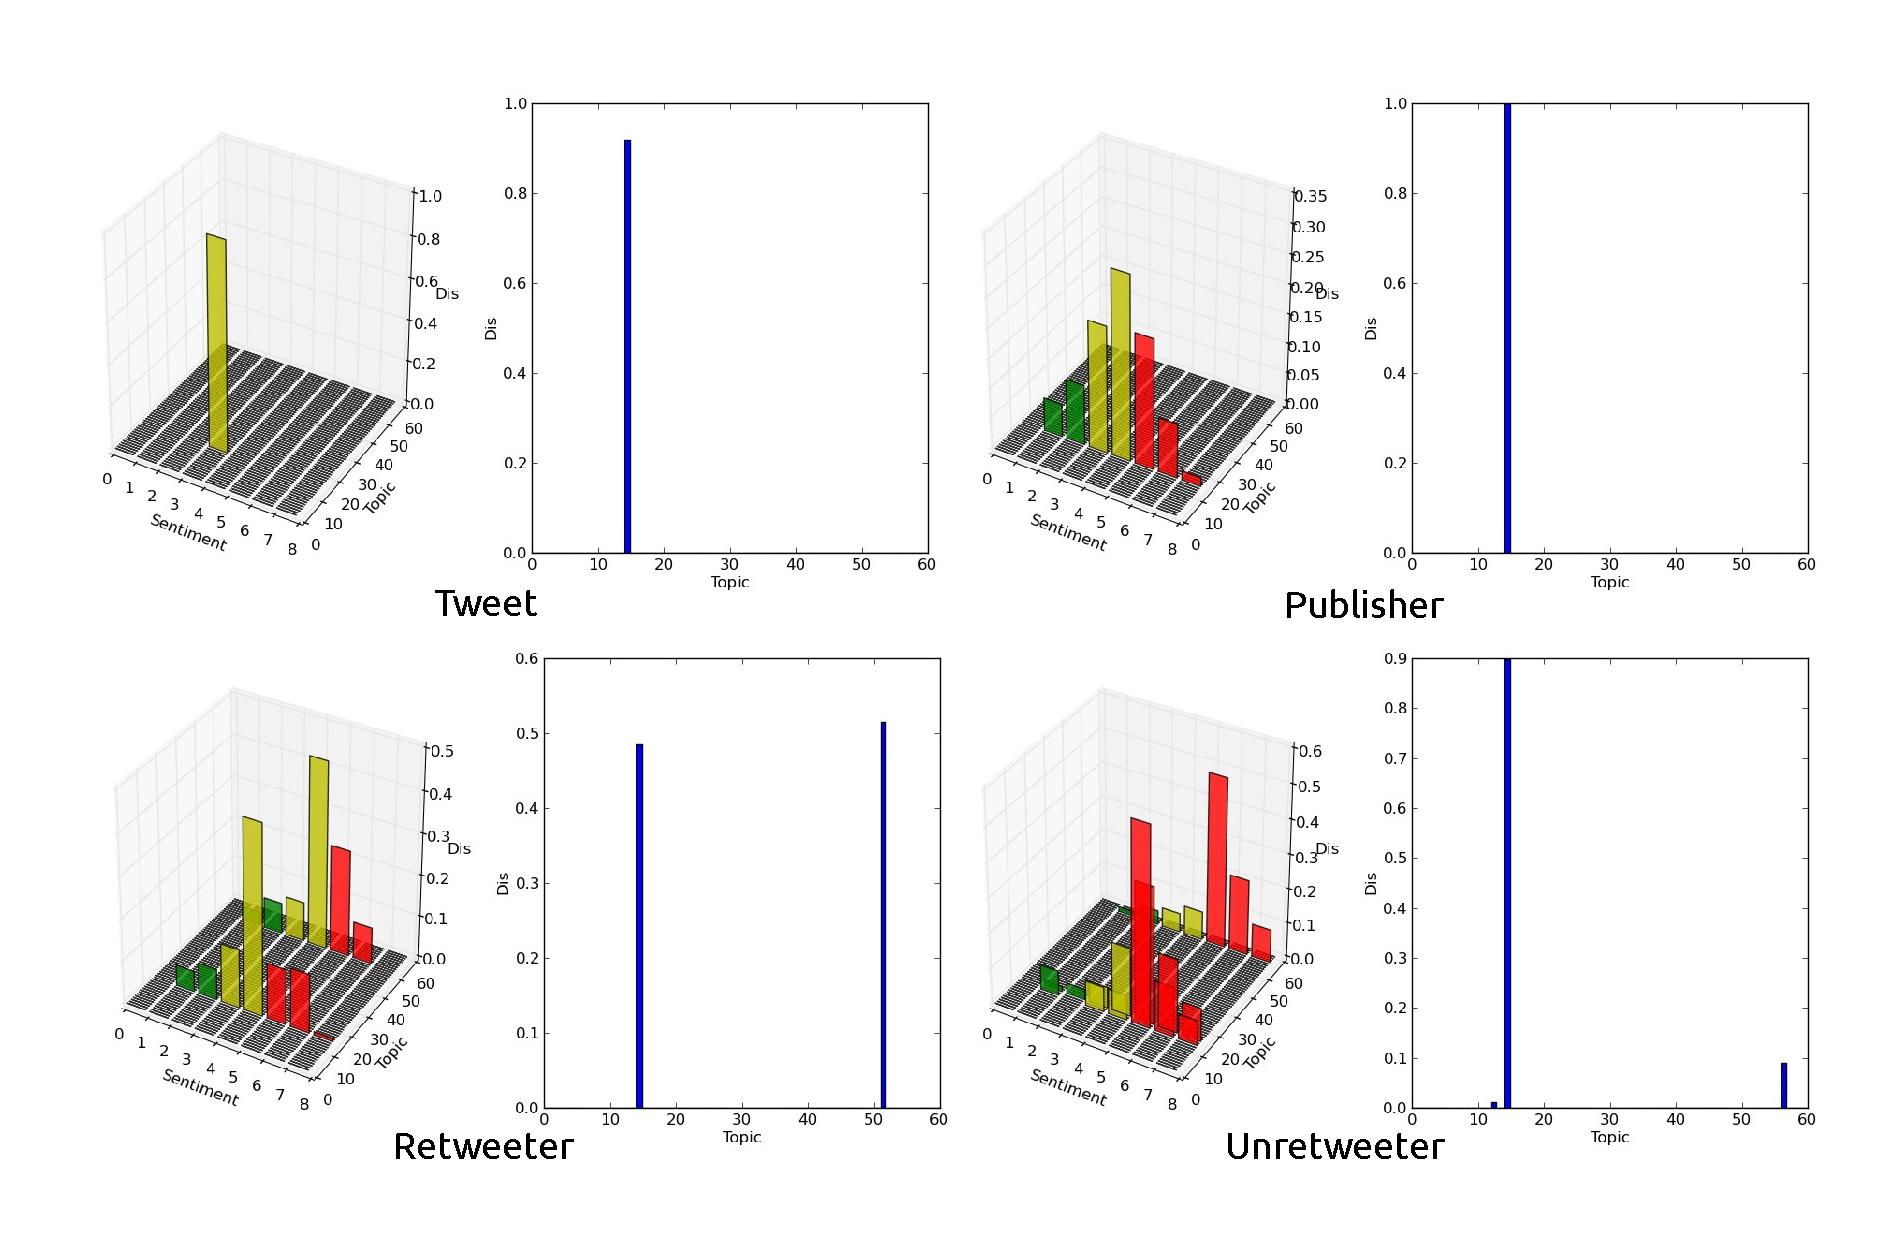
\includegraphics[width=6.0in,height=3.5in]{tweets10.pdf}
%%\vspace{-4em}
%\caption{subjectivity model examples.}
%\label{fig2}
%\end{figure*}
%Figure~\ref{fig3} shows top words of the 14th topic, the tweets of author and followers with word cloud\footnote{We use TagCrowd (\url{http://tagcrowd.com/}) to produce word cloud.}.
%\begin{figure}[htb]
%%\setlength{\belowcaptionskip}{-0.2cm} 
%\centering
%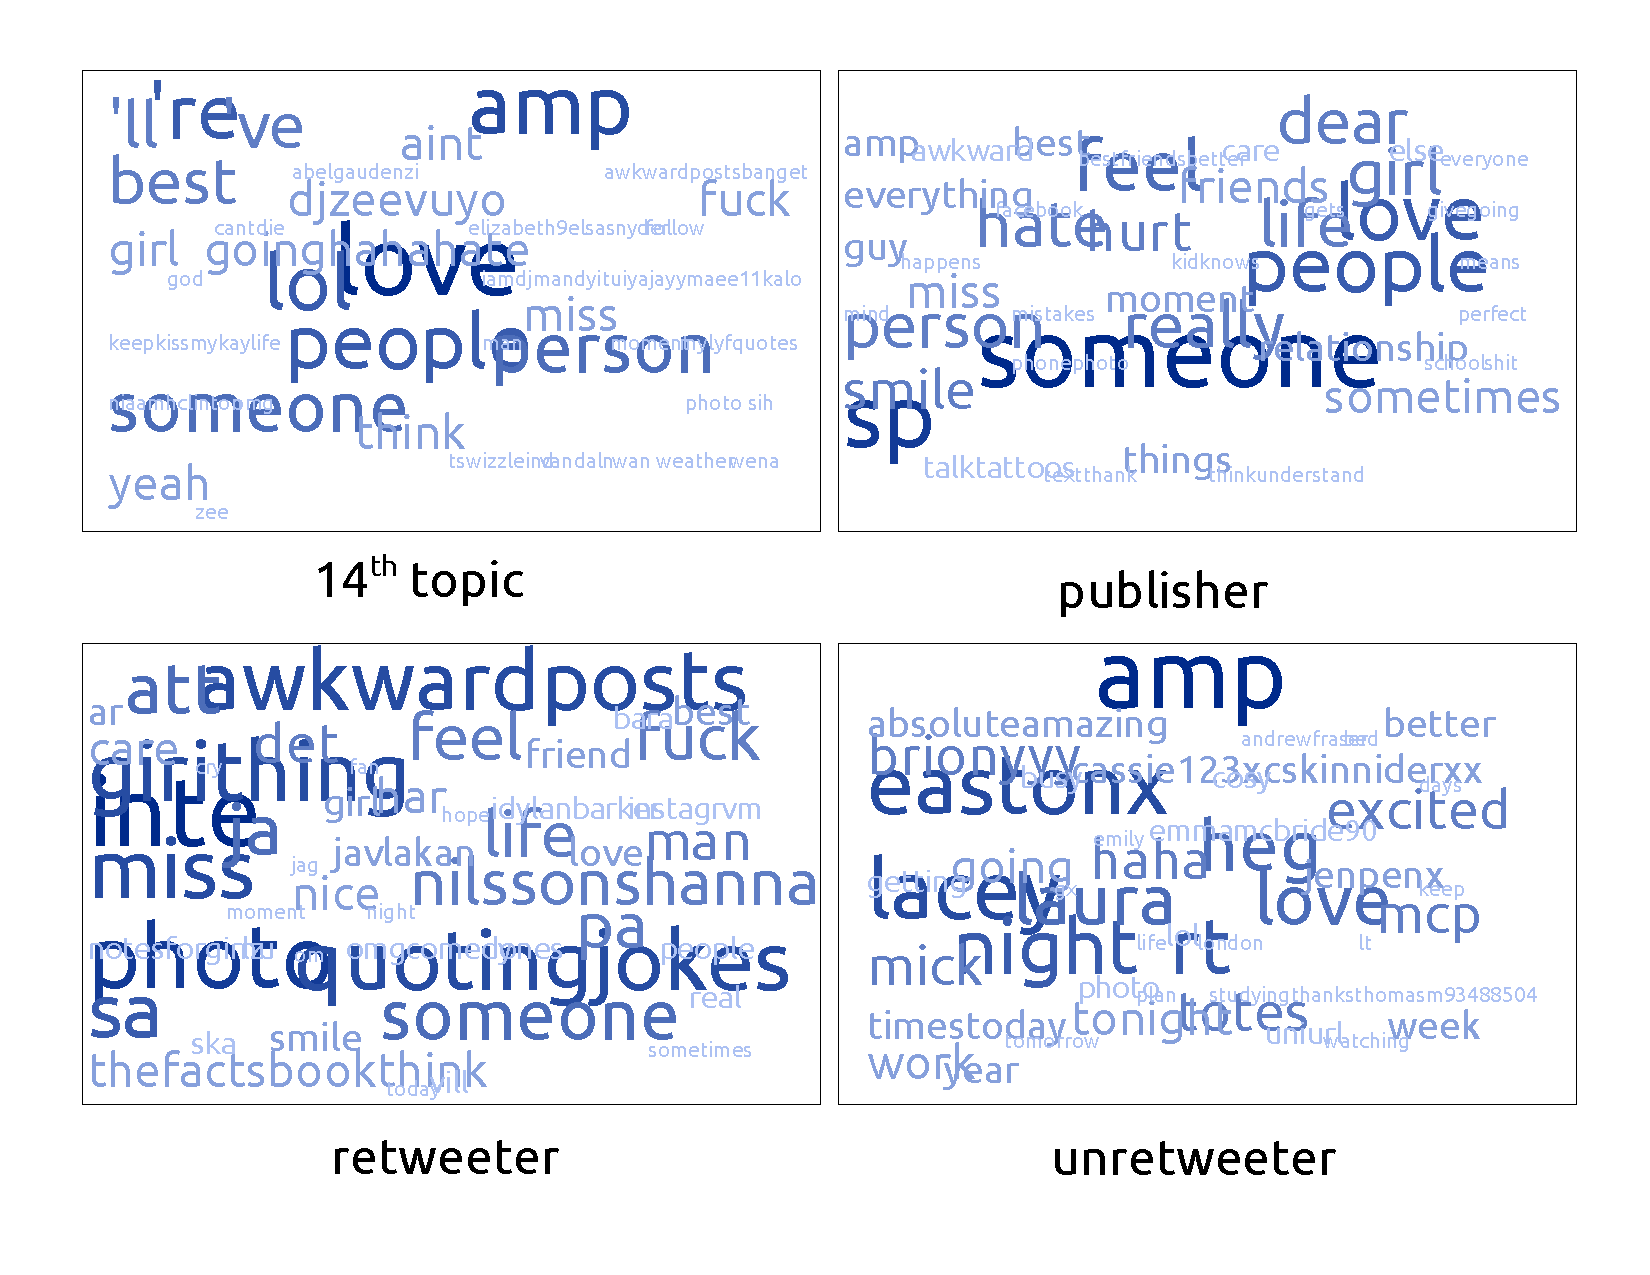
\includegraphics[width=3.5in,height=2.2in]{text_cloud.pdf}
%%\vspace{-3em}
%\caption{Word cloud of 14th topic, publisher and followers}
%\label{fig3}
%\end{figure}
%Content of the tweet is:\\
%\textit{Tweet: ``Sometimes the right person for you was there all along. You just didn't see it because the wrong one was blocking the sight''} \\
%The topic of this tweet is about ``love between people'' and the opinion is neutral, which is in accordance with the 14th topic word cloud in Figure~\ref{fig3} and sub-figure of tweet in Firgure~\ref{fig2}.
%The author concentrates on the 14th topic, and his opinions are mainly neutral (as Figure~\ref{fig2},~\ref{fig3} show).
%As for two followers, the ``retweeter'', has published tweets about two topics (the 14th and 52nd topic) uniformly and his opinions towards the two topics are mainly neutral.
%While the ``unretweeter'', has also talked about two topics (14th and 56th topic), but he is mainly interested in 14th topic and has positive opinion.
%Although two followers have same interest (the 14th topic), their different opinions elicit their different decisions, which verify the subjectivity model can help better understand the retweeting motivation by modelling not only topics but opinions.

\section{Related Work}
\label{relatedwork}
   
User modelling provides insights into user's online behaviors. 
Hannon \emph{et al.}~\shortcite{hannon2010recommending} proposed that Twitter users can be modeled by tweets contents and the relation of Twitter social networks, while content-based approach can find similar users who are "distant" without following relations. 
Macskassy and Michelson~\shortcite{macskassy2011people} discovered user's topic-of-interest by leveraging Wikipedia as external knowledge to determine a common set of high-level categories that covers entities in tweets. 
Ramage \emph{et al.}~\shortcite{ramage10microblogs} made use of topic models to analyze Twitter contents at the level of individual, showing improved performance on tasks such as post filtering and user recommendation. 
Xu \emph{et al.}~\shortcite{xu2012modeling} proposed a mixture model which incorporated three important factors, namely breaking news, friends' timeline and user interest, to explain user posting behavior.
Pennacchiotti and Popescu~\shortcite{pennacchiotti2011machine} proposed a most comprehensive method to model Twitter user for user classification, confirming the value of in-depth features by exploiting the UGC.
A large body of studies have analyzed characteristics of retweeting \cite{macskassy2011people,Luo:2013RMF}, examining factors that lead to increased retweetability \cite{suh2010want,comarela2012understanding} and designing models to estimate the probability of being retweeted \cite{petrovic2011rt,jenders2013analyzing,pfitzner2012emotional}. However, none of the above works have considered the subjectivity of users, who are subjective initiative individuals in behavior-taking. We have fisrtly proposed a novel subjectivity model for users' retweeting behavior analysis. 

\section{Conclusion}
In this paper, from the point of motivation, we postulate that online behaviors of social media users are impacted by their subjectivity. Therefore, we propose a novel model by combining topics and opinions to model the subjectivity of users, which we name as subjectivity model. We design an algorithm for the establishment of subjectivity model, and to make it more efficiently, we consider only the users in an ego network instead of global network and propose a Local Topic Space concept according to the homophily principle. We design novel subjectivity similarity measurement in terms of topic simlarity and opinion similarity. The subjectivity model is applied to the retweeting behavior analysis with three subjecivity similarities among a tweet, its author and followers. 
Experiment results demonstrate the effectiveness of our model for the retweeting analysis problem and show that subjectivity model is able to reach better understanding of retweeting behavior. 

In the future, we will apply the subjectivity model to other social network analysis task such as link prediction and friend recommendation. 

\bibliographystyle{aaai}
\bibliography{subjectivity}

\end{document}
